\section[The Waterfall Target]{The Waterfall Target
\footnote{
  $ CVS~revision~ $Id: waterfall-target-old.tex,v 1.2 2003/12/13 06:23:39 gen Exp $ $
}
\footnote{Authors: Dr.No \email{????@jlab.org}}
}

The waterfall target system provides a target for experiments on 
$^{16}$O (see figure \ref{fig:uno}). 
The conceptual design of the waterfall target system for Hall A  is
very similar to the one used at Saclay \cite{Garibaldi:1992mb}.
The thickness of the waterfall target can 
be modulated by changing the pump speed; this 
adds flexibility to the system and allows the user to choose the best
value according to the wanted resolution and luminosity.

The hydrogen in the water can be used for calibration purposes.
Elastic scattering  from the hydrogen in the target can be used to 
measure and monitor the target thickness. The counting rate in the elastic
peak is directly proportional to both the beam current and 
the target thickness.

\begin{figure}[htbp]
\begin{center}
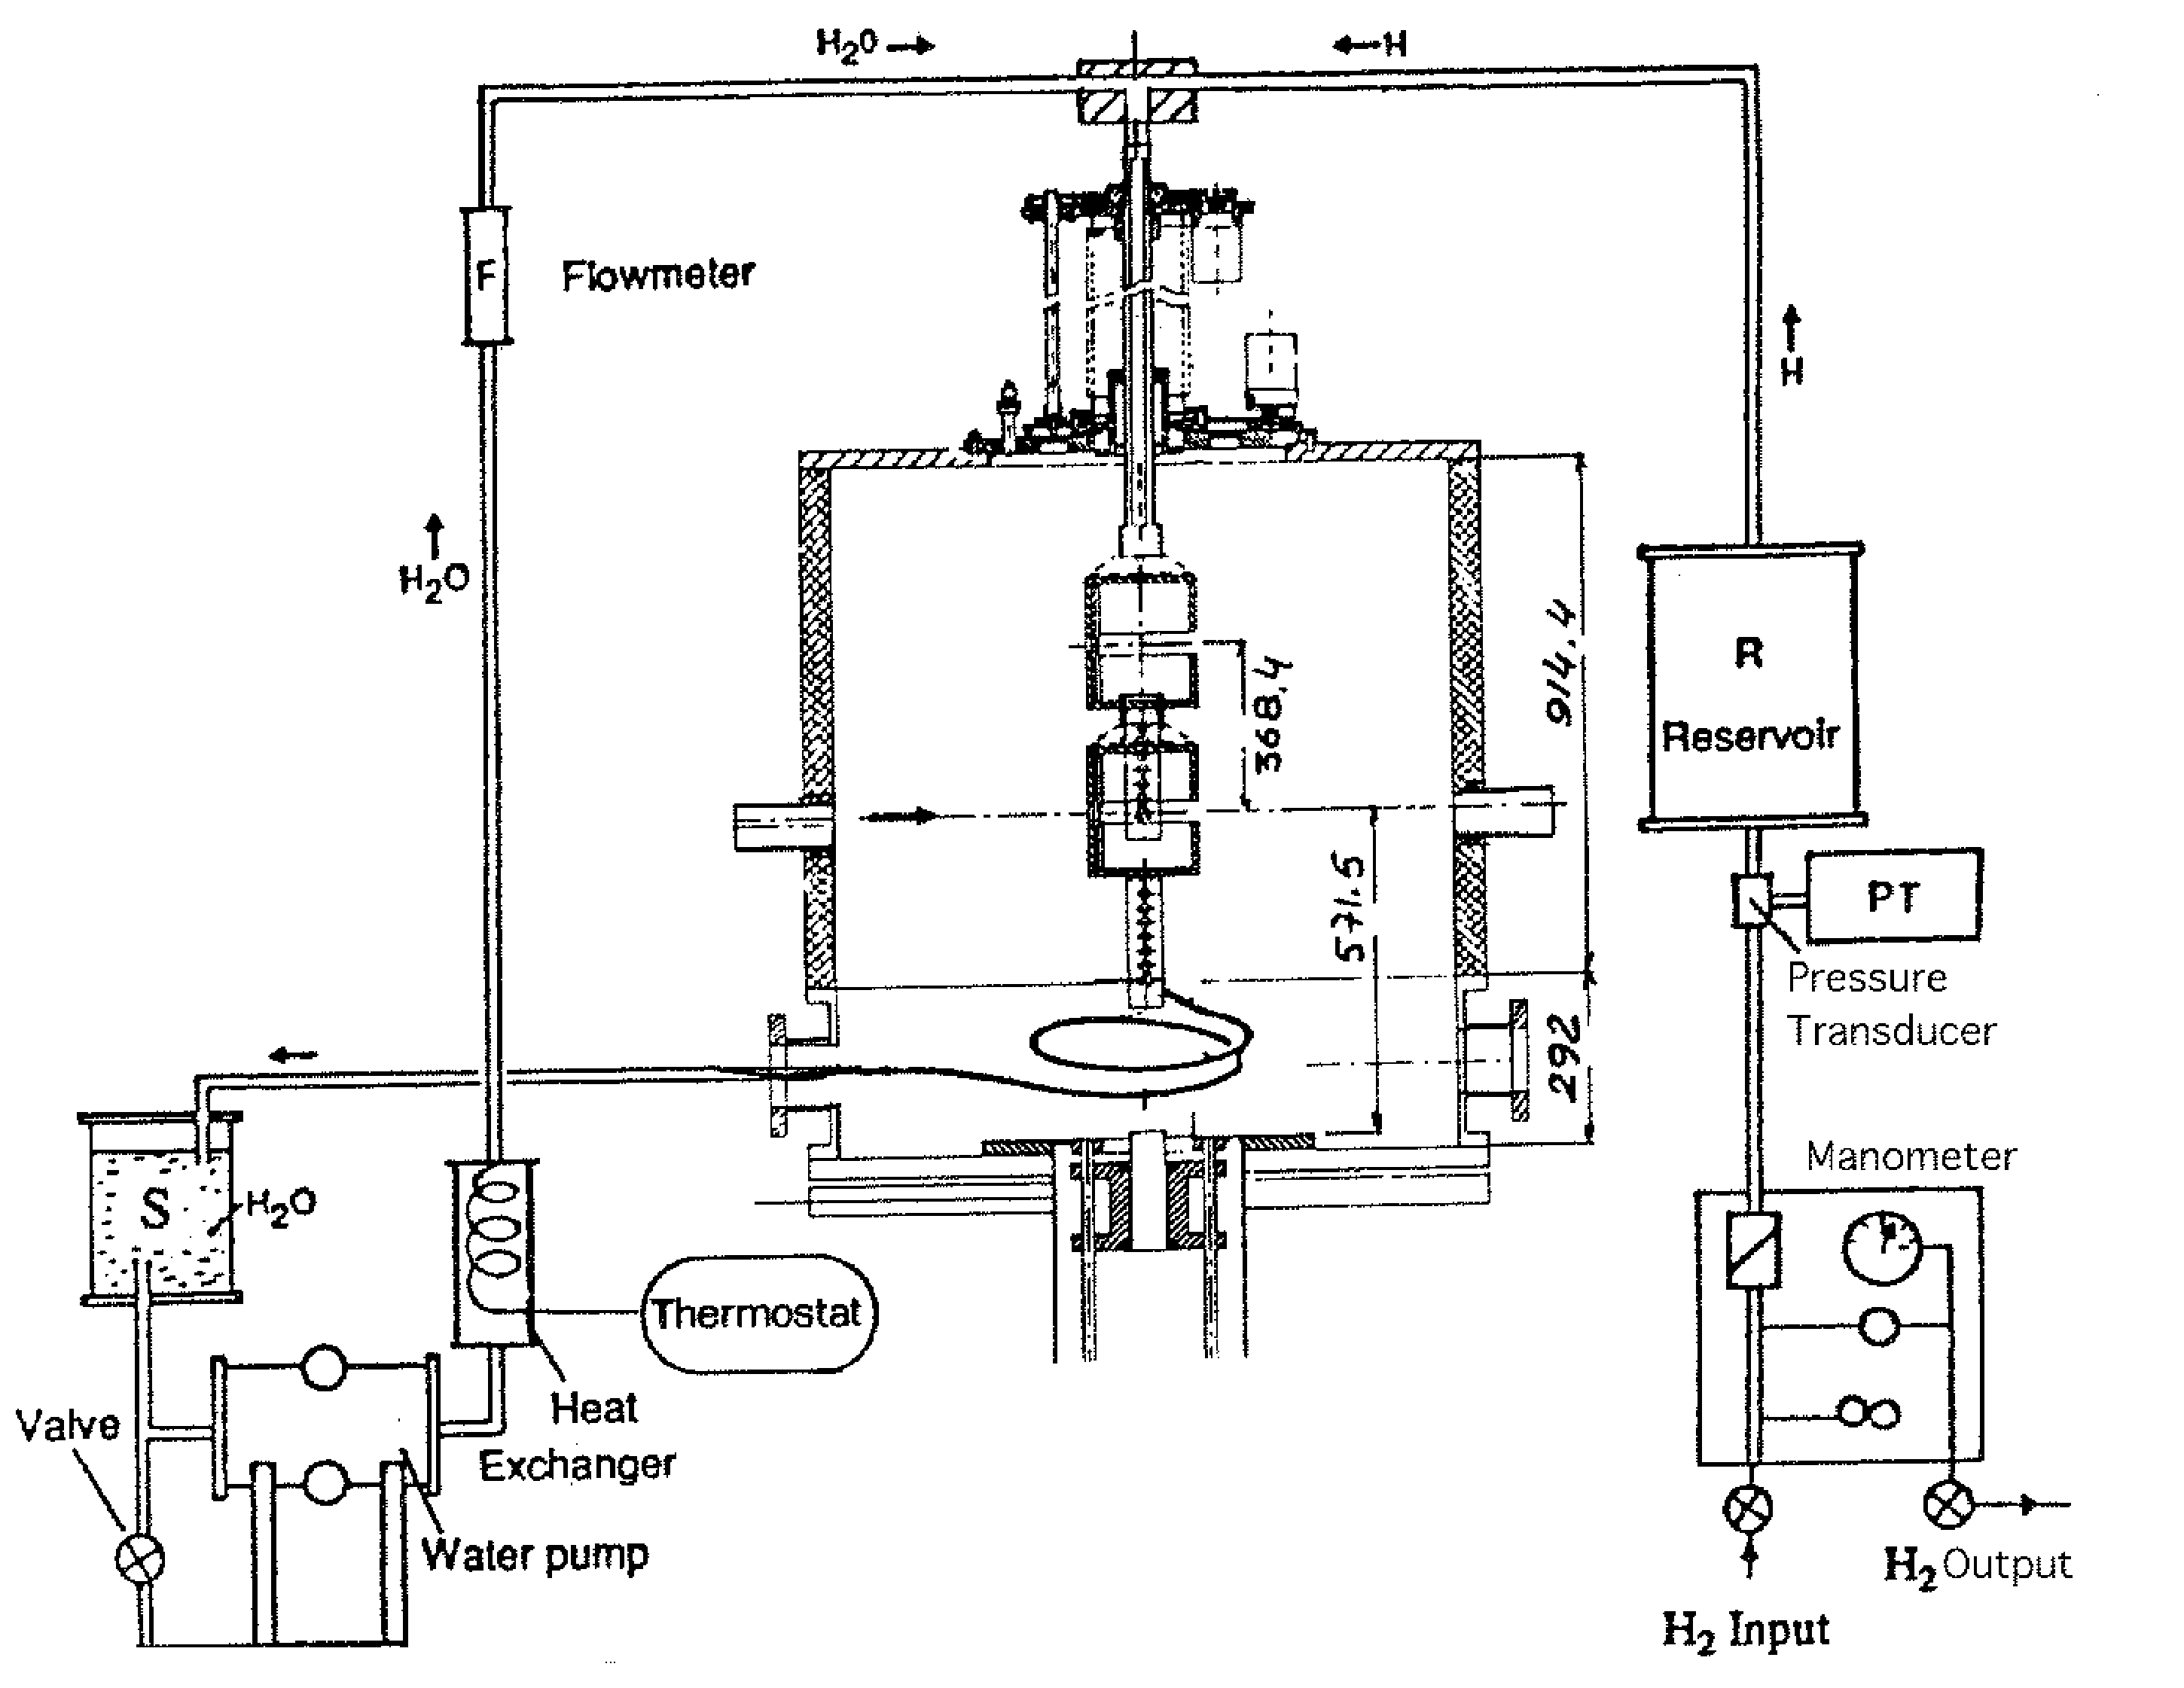
\includegraphics[angle=0,width=14cm,clip]{wf1_ber_uno}
\caption[Waterfall Target System]{The target system.}
\label{fig:uno}
\end{center}
\end{figure}


The waterfall target can be single foil or multi-foils according to
the need of the particular experiment. In fact, a modified version of this 
target has been built  and used for experiments at NIKHEF (a
$\sim 150$ mg/cm$^2$ single-foil and a three-foil one 
$\sim 60 \times 3$ mg/cm$^2$). 
The target built for Jefferson Lab Hall A for the two commissioning 
experiments on $^{16}$O (E89003 and E89033) is a three-foils  one  with 
thickness ranging from $\sim 130-200$ mg/cm$^2$ for each foil, 
depending on the pump speed. 

The main components of the target system are:
\begin{enumerate}
\item The waterfall target container, also referred to as ``target cell'' in this document;
\item The solid target ladder and the solid targets; 
\item The hydraulic system;
\item The gas system;
\item The movement system;
\item The slow-control system.
\end{enumerate}

The waterfall foils are produced inside the waterfall target container,
which is mounted in the standard Hall A scattering chamber. 

The water, continuously pumped from a reservoir, goes through a heat exchanger
into the target zone, and then back into the reservoir. All parts in contact 
with the water are made of stainless steel. In the target zone, the water pressed through a system of slits and holes and guided by the stainless steel bars
forms one or more flat rectangular films,
which are stable due to the surface tension and to the adherence to the guiding bars.

The thickness of the foil(s) is (to some extent) a function of the 
pump speed which determines the flow rate.  
Once the foil is formed (there is a 
minimum value of the pump speed/flow rate for this, depending on the 
particular target) the thickness increases with the pump speed. The 
maximum pump speed depends essentially on the dimensions of the
slits and holes the water passes through. 

An absolute calibration of the target thickness as a function of the
 pump speed needs to be done before the experiment.
One way of measuring the absolute target thickness 
is to  measure the raw counting rate in the spectrometer.

The target used for E89003 and E89033 was at a fixed angle during the 
experiments. Therefore the waterfall target container is designed as a box
with dimension of $630\times68\times8$ mm$^3$. 

The entrance and exit windows of the target cell are 
circular (40 mm in diameter) and are made of gold-plated Be (75 $\mu$m thick)
(Fig. \ref{fig:wf1_cell1}, \ref{fig:cell2}).
Scattered particles go through the `lateral' windows, made of 
stainless steel (25 $\mu$m thick, dimension of ~320 X 8 mm$^2$).
Some schematic views of the target container are shown 
in Figures \ref{fig:wf1_cell1},
\ref{fig:cell2}, \ref{fig:cell3a} and \ref{fig:cell3b}. 

\begin{figure}[htp]
\begin{center}
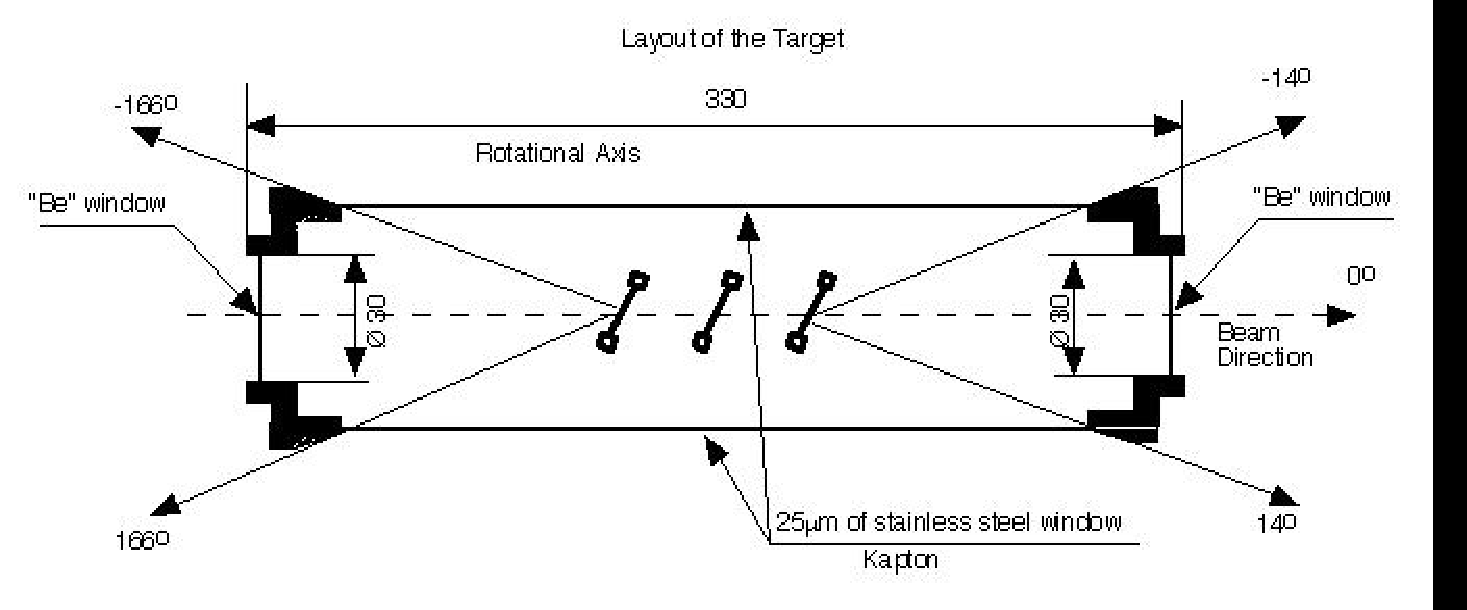
\includegraphics[angle=0,width=12cm,clip]{wf1_ber_cell1}
\caption[Waterfall Target: Cutaway of Target Cell]{A cutaway of the waterfall target cell.}
\label{fig:wf1_cell1}
\end{center}
\end{figure}

\begin{figure}[htp]
\begin{center}
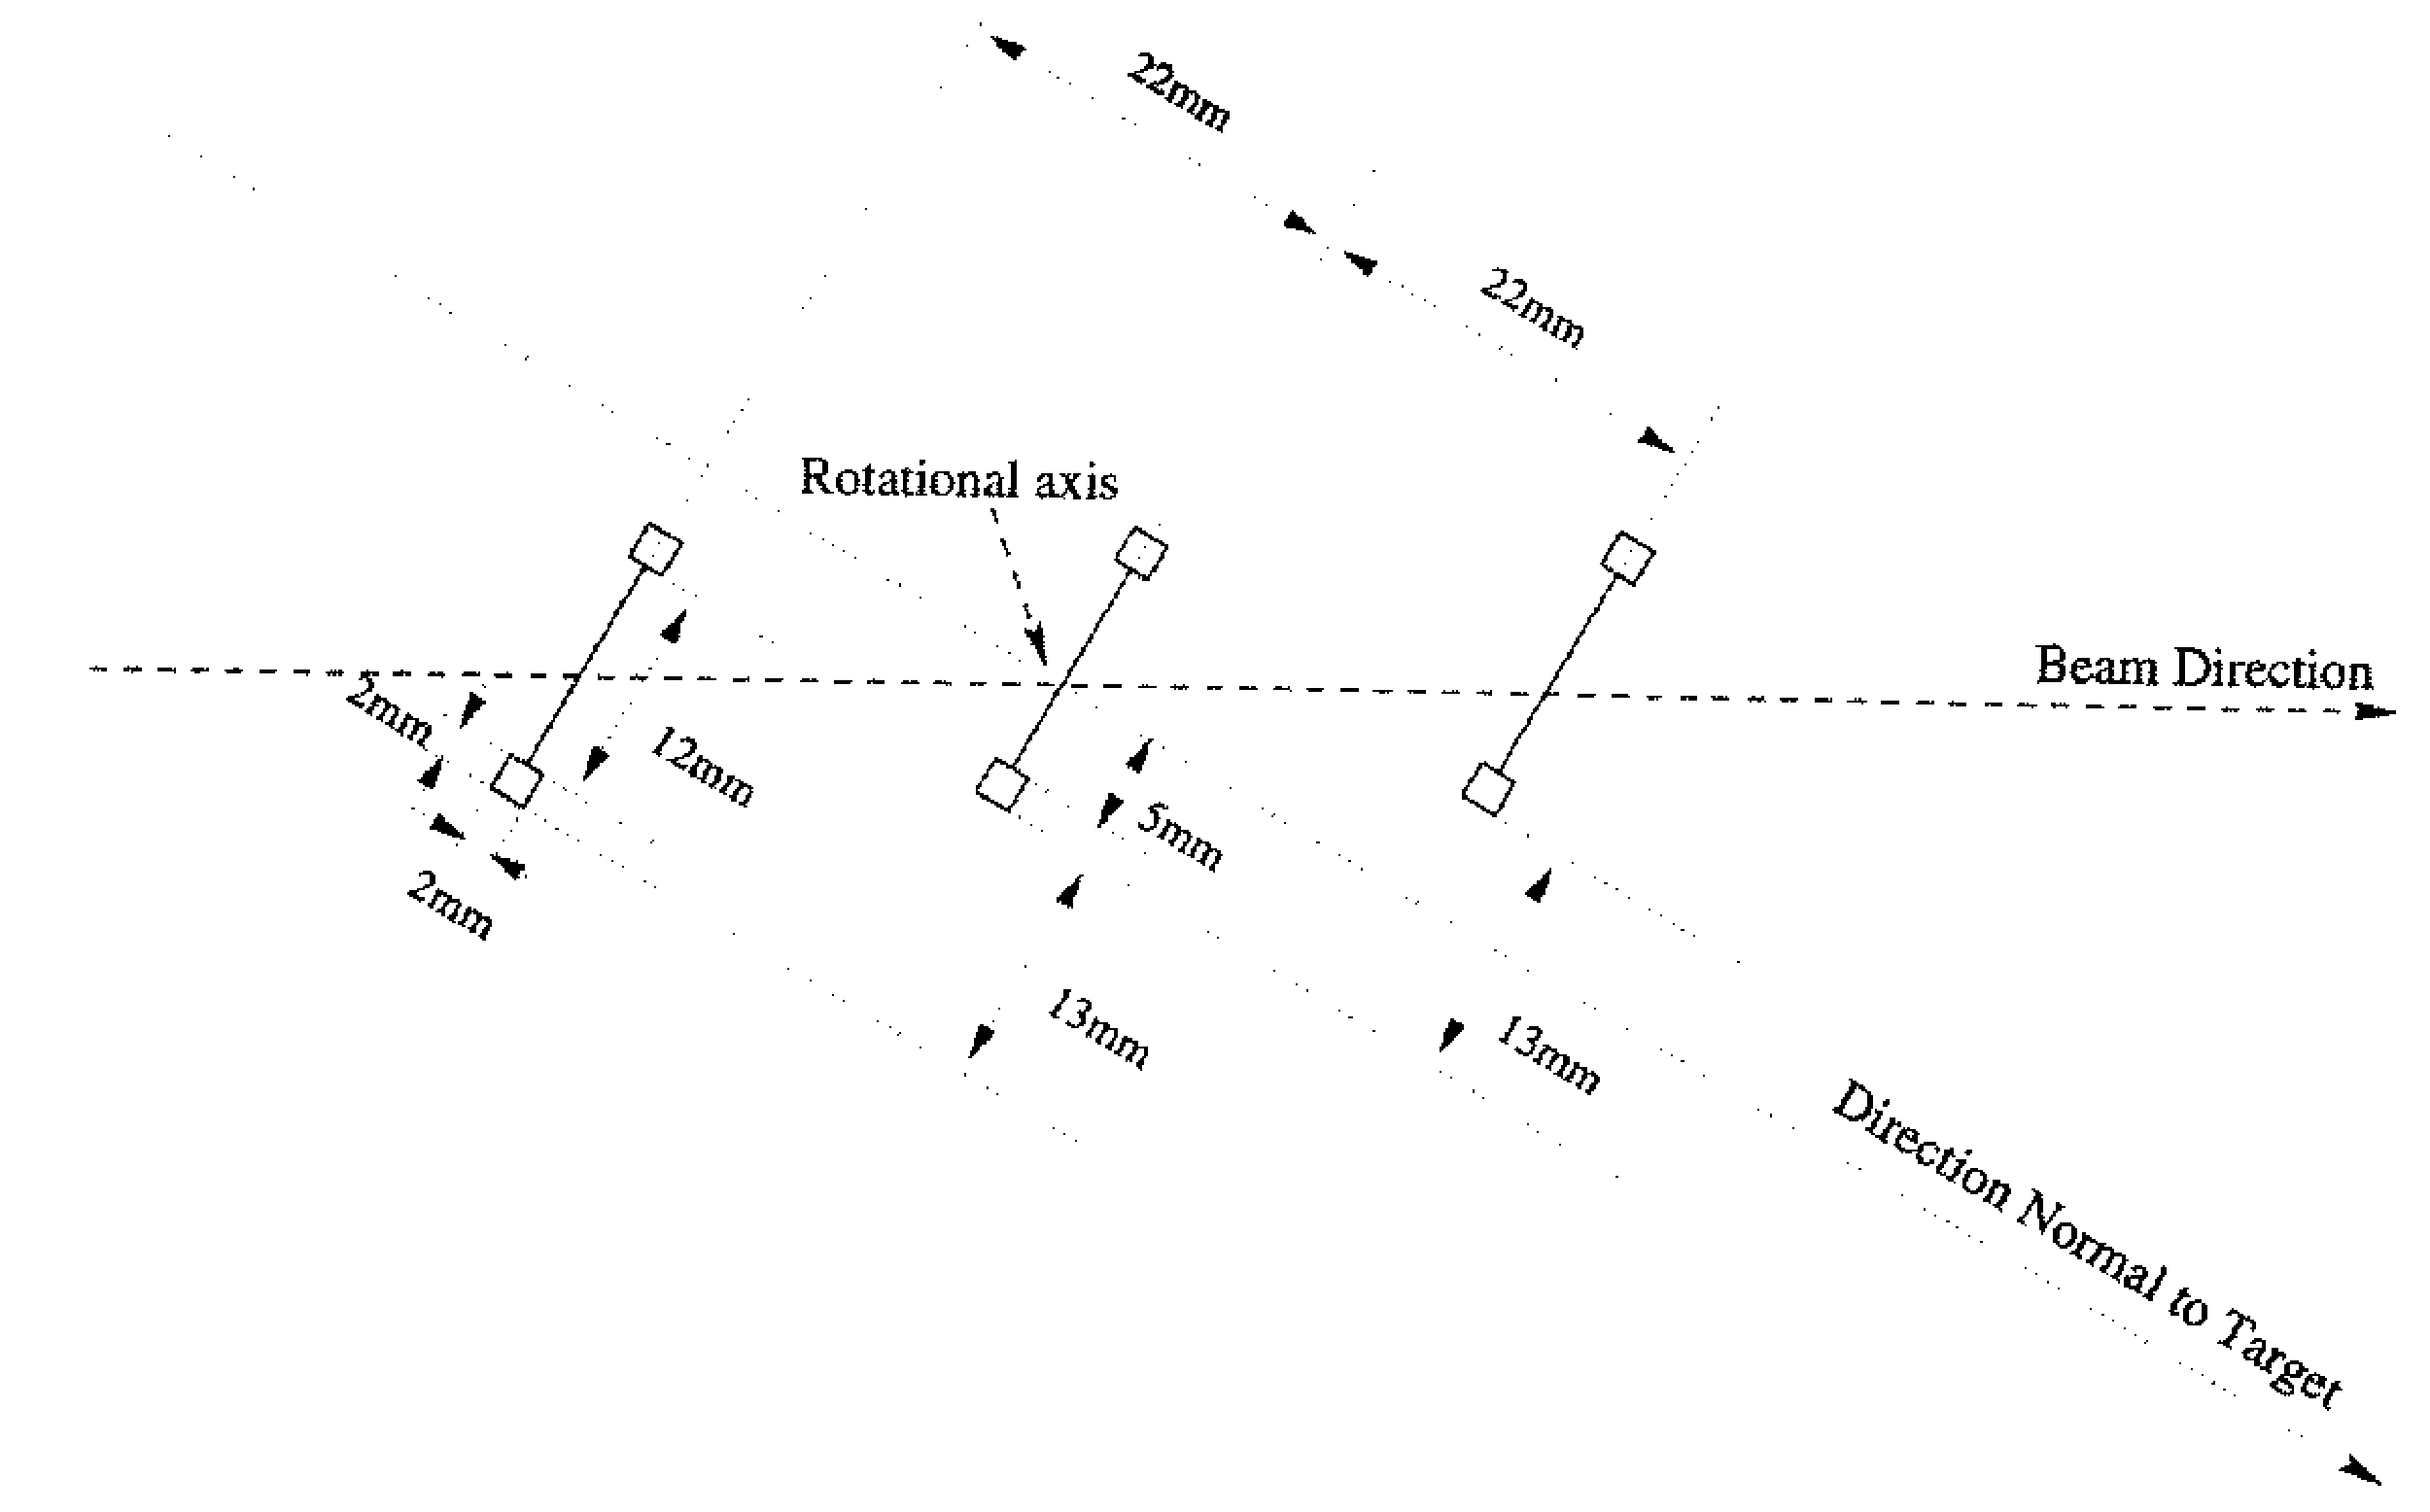
\includegraphics[angle=0,width=12cm,clip]{wf1_ber_fig2}
\caption[Waterfall Target: Three Foil Geometry]{Detailed view of the 3-waterfoils geometry.}
\label{fig:cell2}
\end{center}
\end{figure}

\begin{figure}[htp]
\begin{center}
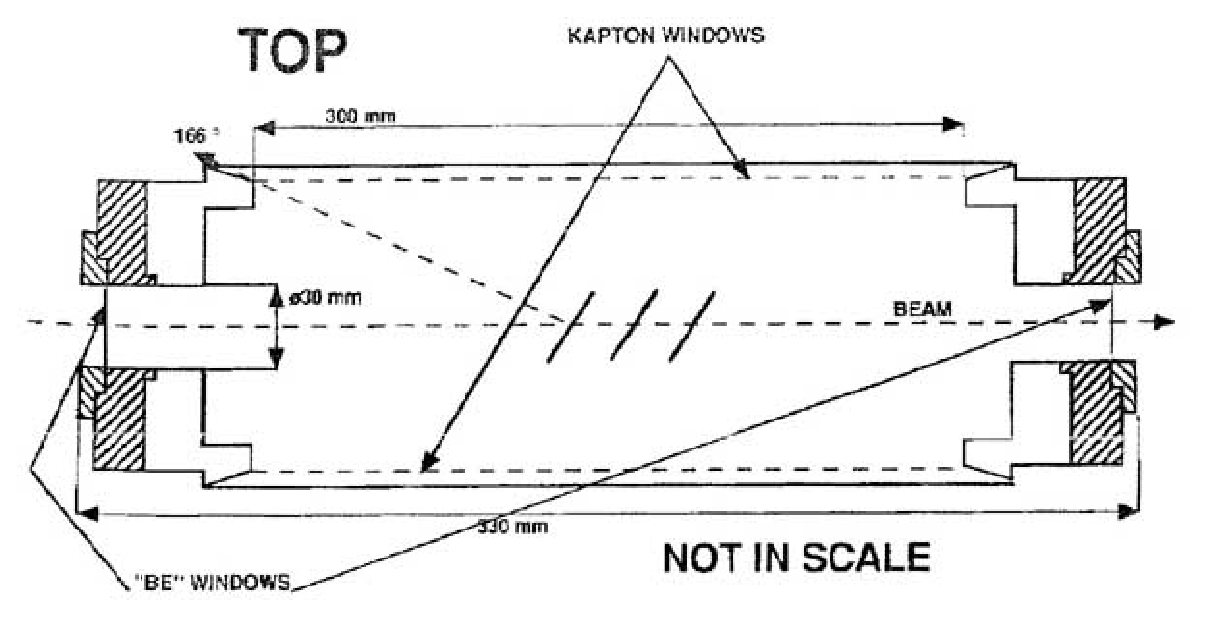
\includegraphics[angle=0,width=15cm,clip]{wf1_fig3a}
\caption[Waterfall Target: Target Container]{Cutaway view of the waterfall target container.}
\label{fig:cell3a}
\end{center}
\end{figure}

\begin{figure}[htp]
\begin{center}
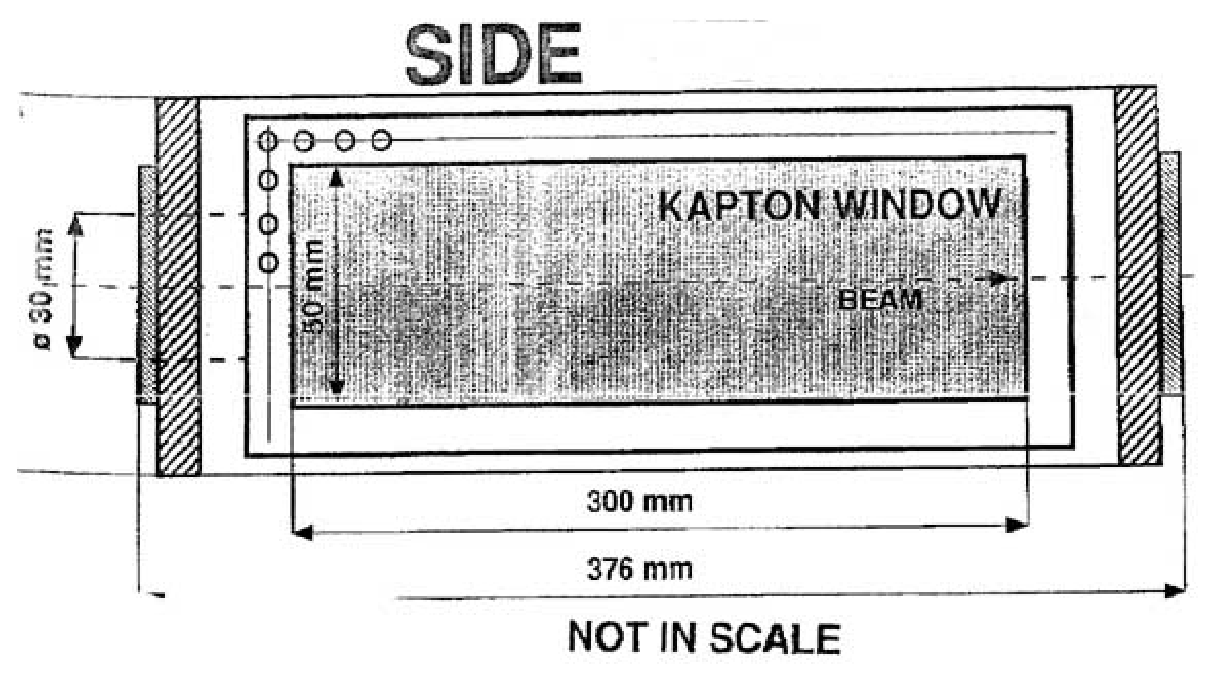
\includegraphics[angle=0,width=15cm,clip]{wf1_fig3b}
\caption[Waterfall Target: Side View]{Side view of the waterfall target container.}
\label{fig:cell3b}
\end{center}
\end{figure}


The three foils are parallel and identical. Each foil is 12 mm wide, 
guided by two poles each of 2 mm by 2 mm cross-section. 
In the direction normal to the target, the foils are 22 mm 
apart. The normal direction of each foil is 30$^o$ with respect to beam line, 
and the normal direction points  towards H-arm. The center of each foil is 
shifted 1 mm along the foil direction and towards E-arm, see Figure 
\ref{fig:cell2}. The tolerance of the 
machining is less than 0.2 mm.  

A solid target ladder is attached to the bottom of the waterfall target 
container, which holds up to 5 solid targets. The 
water coming back to the container goes through two cylinders
in contact with the side of solid target holders, providing some cooling for
solid targets. 

\subsection{The hydraulic system}

The hydraulic system is a closed circuit (loop), see Fig. \ref{fig:uno} and 
\ref{fig:acqua}. Water is pumped from a stainless steel water
reservoir (or tank)
to the target, and then back to the tank through stainless steel tubes.
In order to produce a stable film, a gear  pump, magnetically coupled to a 
dc motor, is used.

A tachometer which is on the pump axis measures the pump speed (turn/min), 
and a flowmeter, which is placed before the entrance of the 
scattering chamber, measures the flow rate. The set
voltage is also read, although it is redundant.
These parameters can be used to
monitor the target thickness stability.

\begin{figure}[htp]
\begin{center}
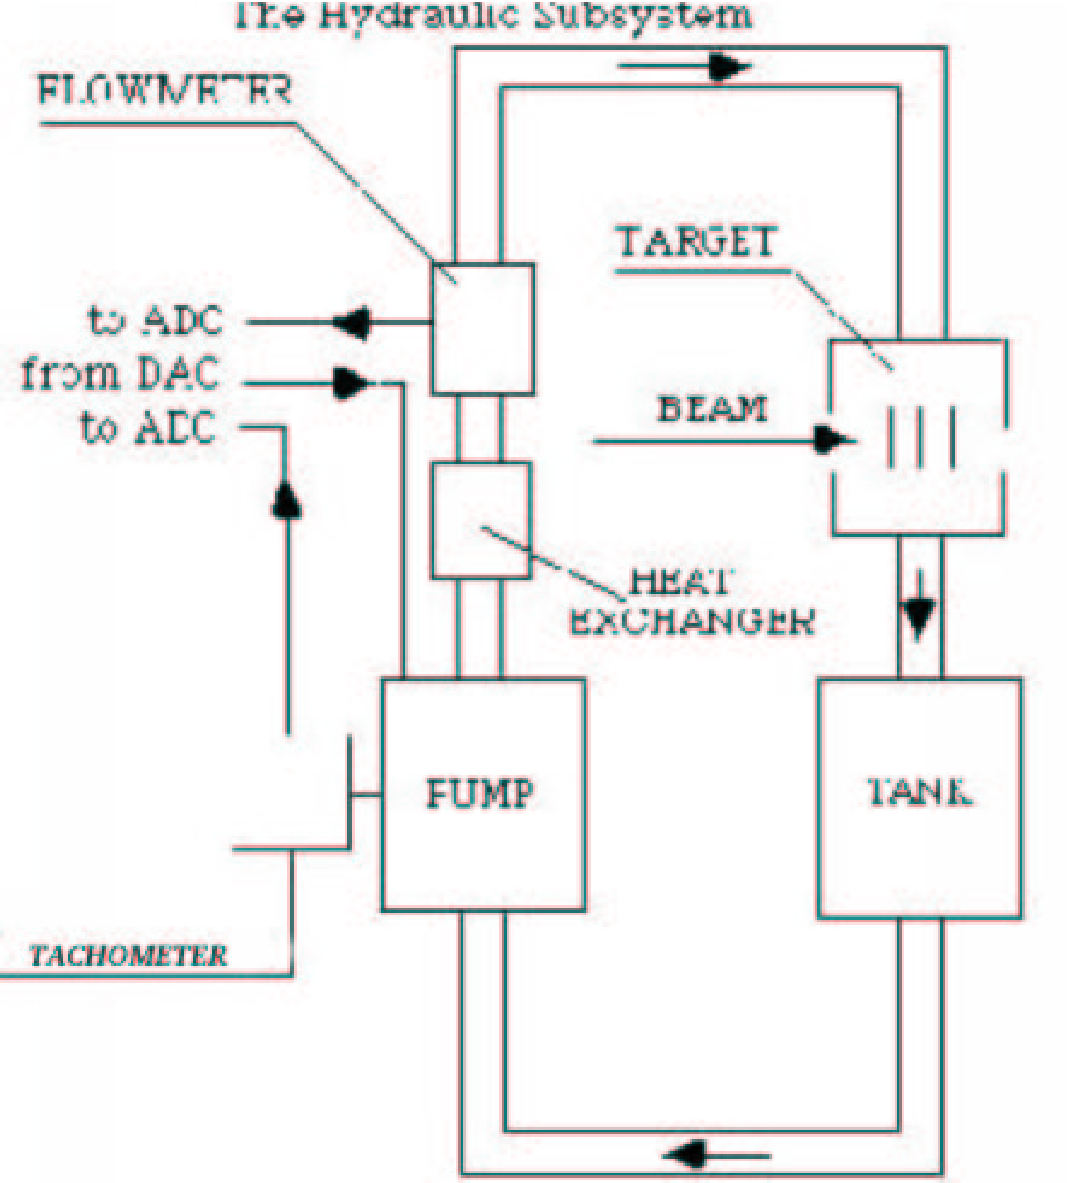
\includegraphics[angle=0,width=15cm,clip]{wf1_fig4}
\caption[Waterfall Target: Hydraulic Schematic]{The Hydraulic system: a schematic view.}
\label{fig:acqua}
\end{center}
\end{figure}


\subsection{The gas system}

The gas system, connected with the hydraulic system,  
is designed to pump gas into the waterfall target container to reduce 
background. Normally hydrogen gas is used. The gas system is made of 
a load and discharge tube circuit to allow the removal of 
the air by flushing the hydrogen into the target cell (and the water 
reservoir). Once the system is full, the circuit will be
closed by electro-valves. 

\subsection{The movement system}

The waterfall target and the solid target ladder can, by design, both 
be rotated around the central axis of the scattering chamber 
and be moved vertically to change the target at the beam 
position. This is done by a mechanical system schematically shown in 
Fig. \ref{fig:uno}, which consists of step motors and absolute optical 
encoders whose precision is 0.1 mm and 0.1 degree.
For E89003 and E89033 experiments, the rotation motion of the target is not
required and thus has been disabled to prevent accidental change of the 
target orientation. 

\subsection{The slow-control system}

The slow control system consists of
two Macintosh computers, two VME crates, an ADC, a DAC and an electronic 
circuit. It handles both the data acquisition and the control of the target
system. The layout is shown in Figure \ref{fig:sette}.

\begin{figure}[htp]
\begin{center}
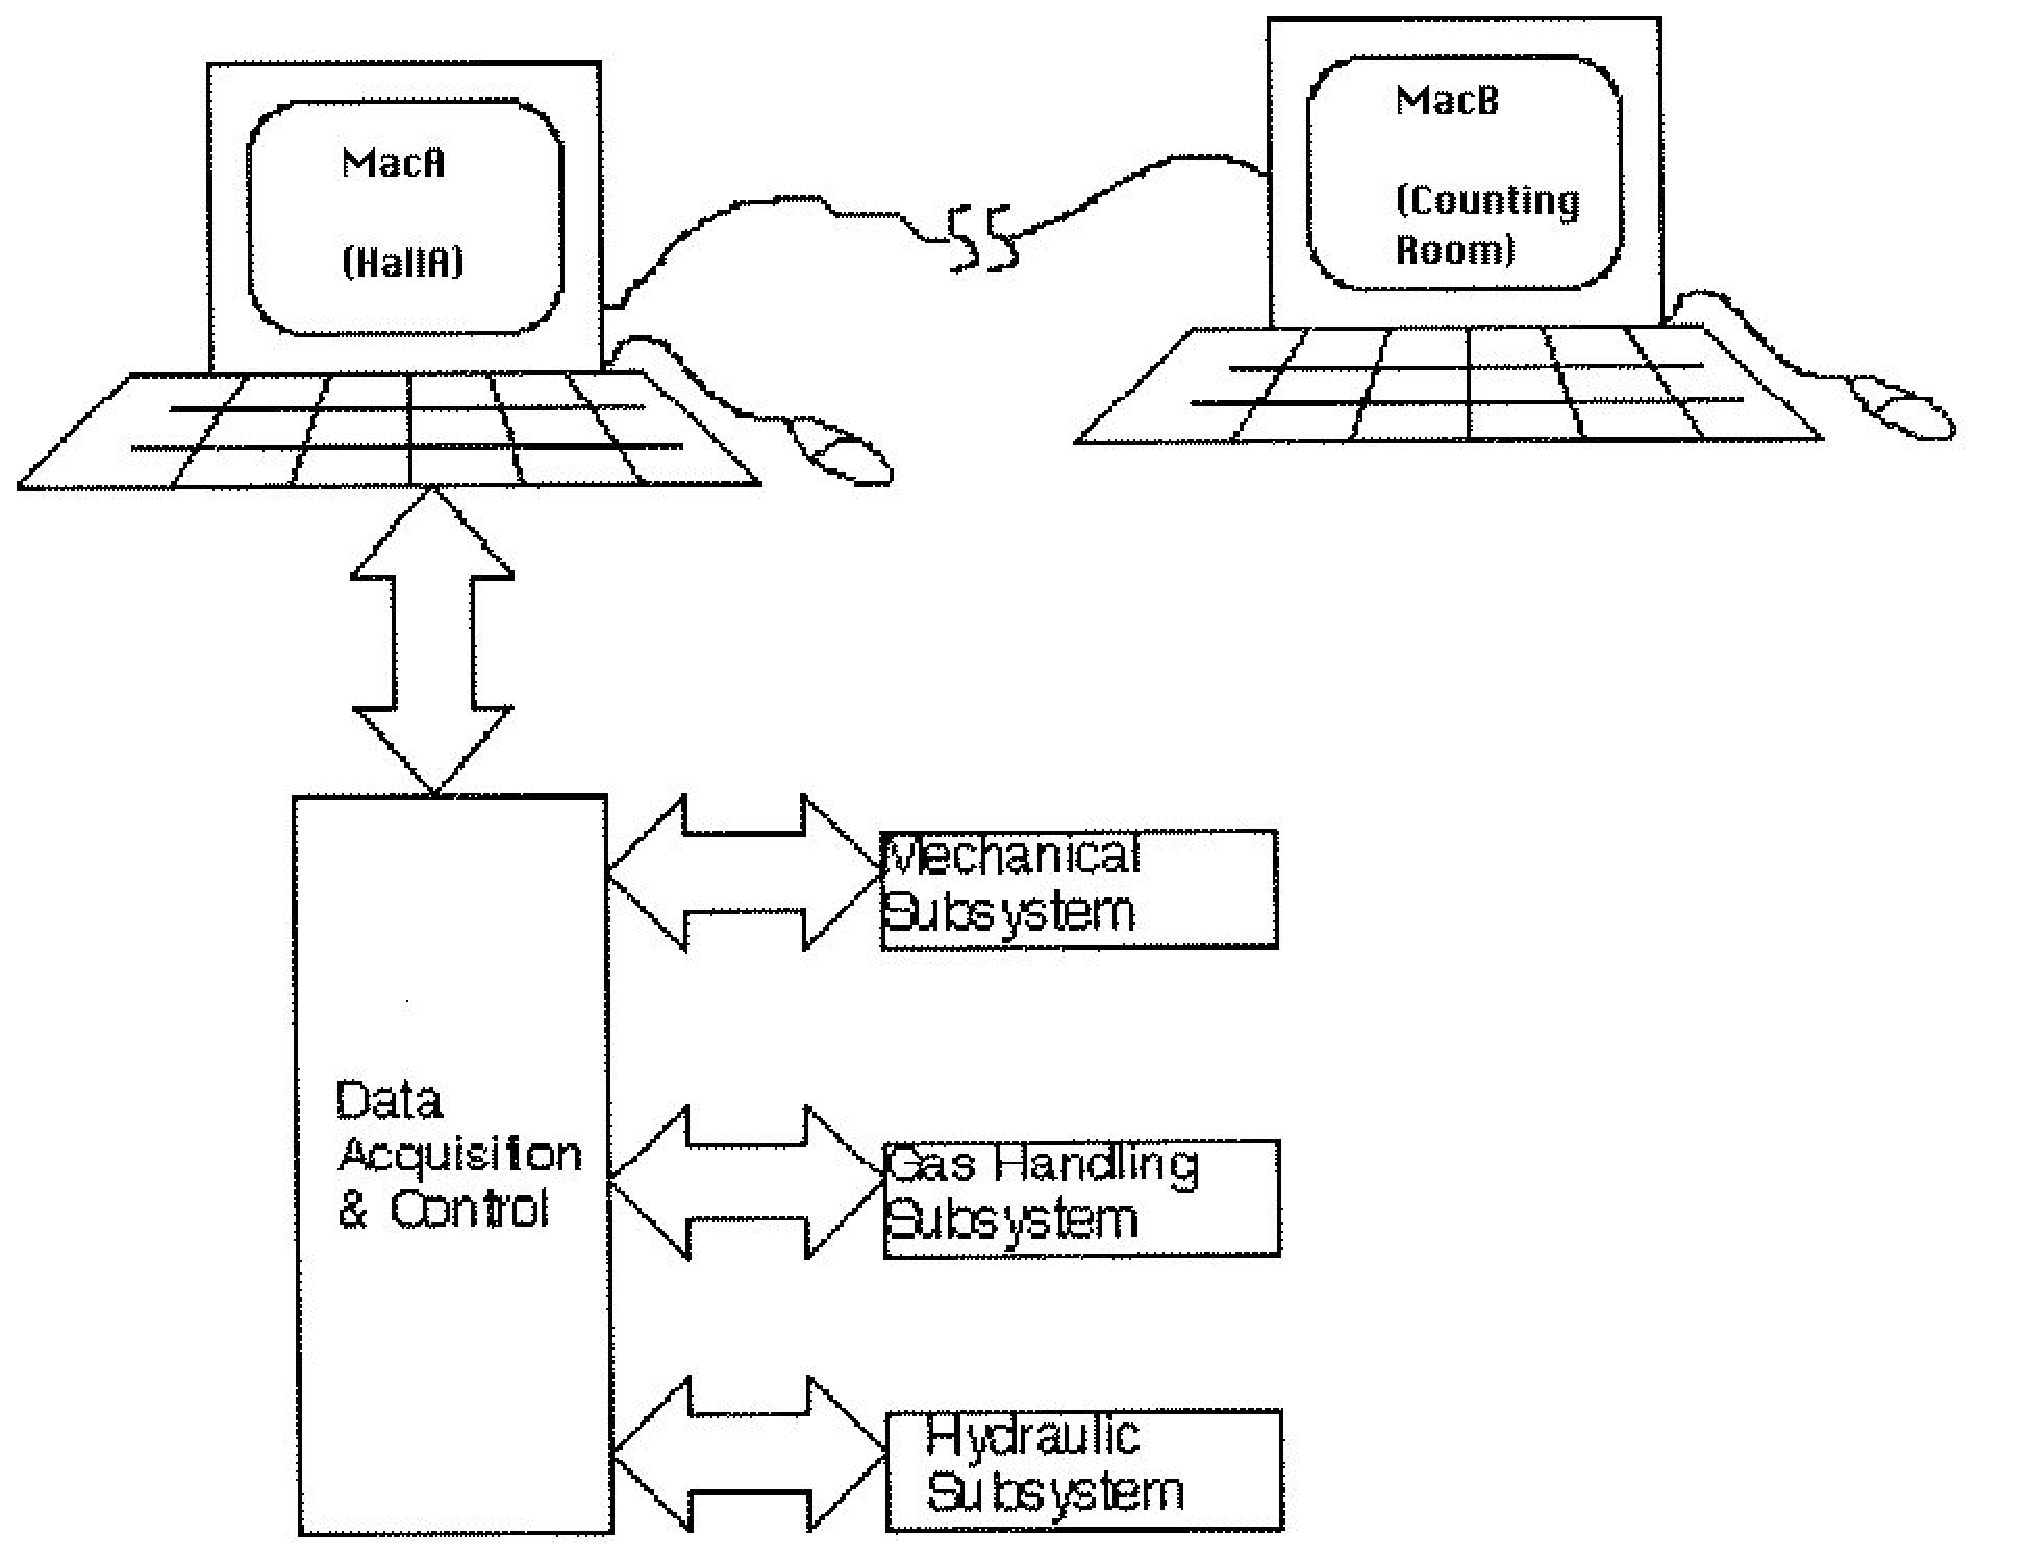
\includegraphics[angle=0,width=10cm,clip]{wf1_ber_fig7}
\caption[Waterfall Target: Schematic]{Schematic view of the whole system.}
\label{fig:sette}
\end{center}
\end{figure}

Each Macintosh computer is hosted by one VME crate. The two computers are
interconnected via an optic ethernet line
(Fig. \ref{fig:control1}, \ref{fig:control2} ). 
The first one (also called MacA) is in the hall. This is the Master.
It controls the electronics directly with the slow-control program H2OCEBAF97 
written in Labview.
The second one (called MacB) is a slave, and is located in 
the counting house where it controls the target system through MacA.

\begin{figure}[hp]
\begin{center}
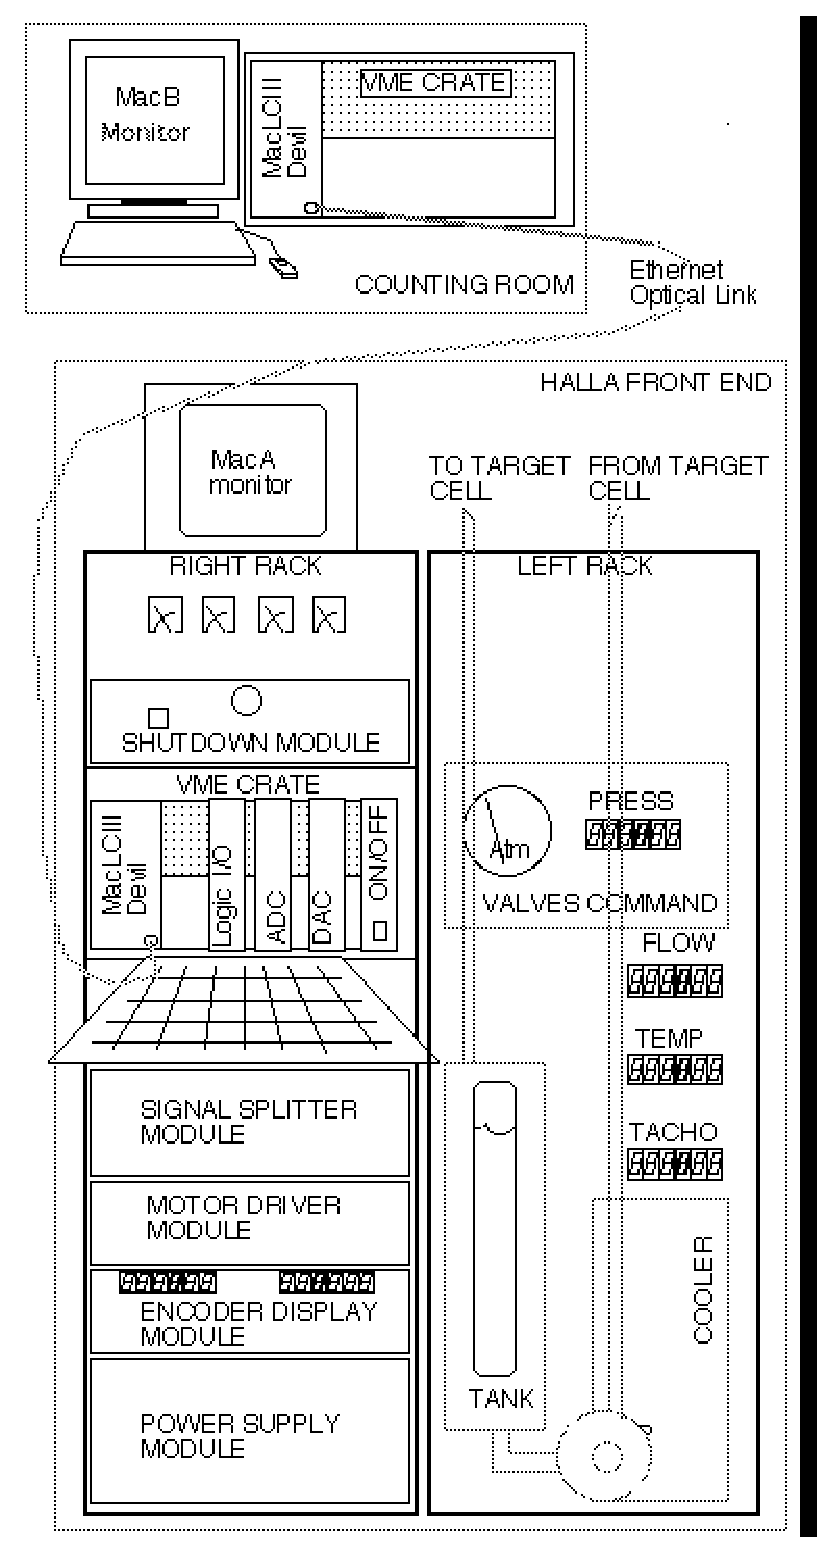
\includegraphics[angle=0,width=10cm,clip]{wf1_ber_fig6}
\caption[Waterfall Target: Slow Controls]{Layout of the slow control system.}
\label{fig:control1}
\end{center}
\end{figure}
 
\begin{figure}[hp]
\begin{center}
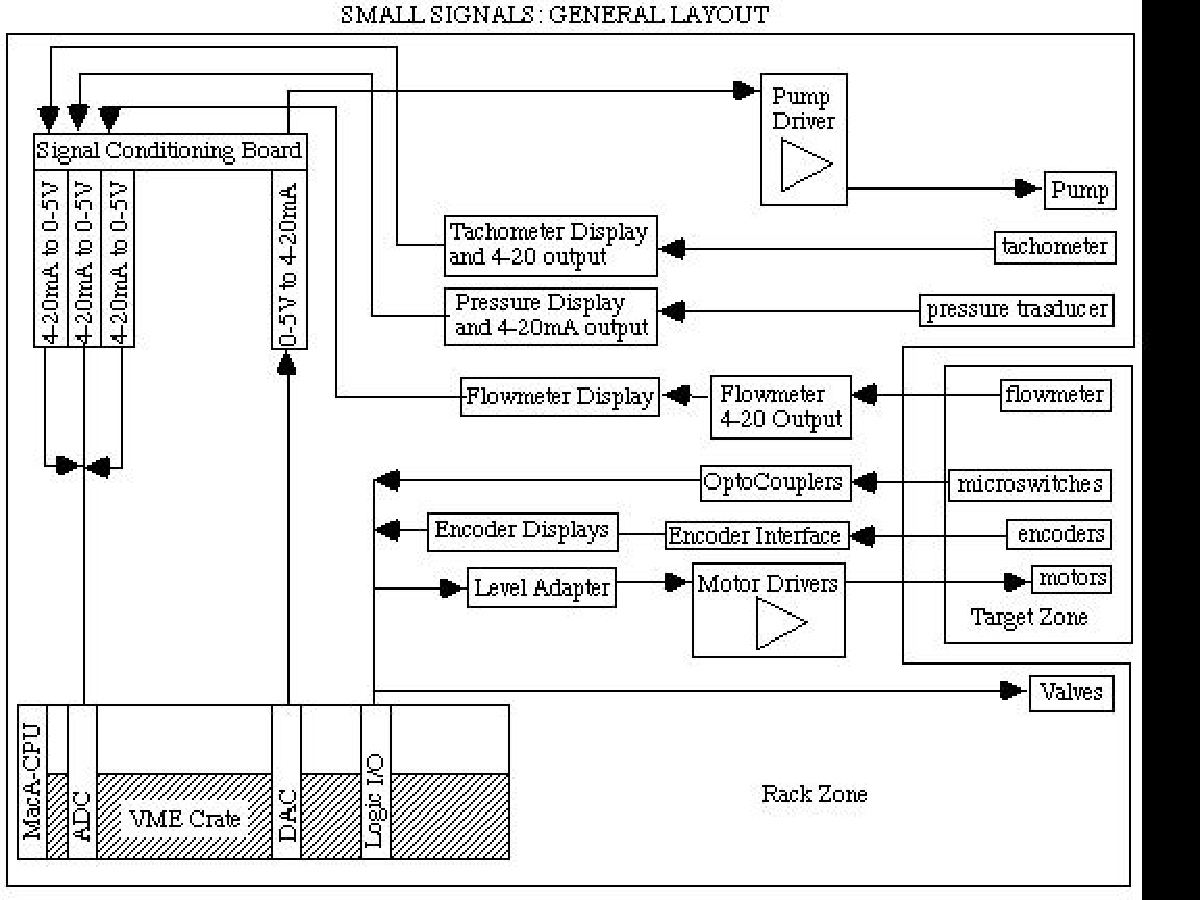
\includegraphics[angle=0,width=13cm,clip]{wf1_ber_fig8}
\caption[Waterfall Target: Signal Layout]{Signals layout}
\label{fig:control2}
\end{center}
\end{figure}


Some of the controls and monitoring can also be done manually. This provides 
an independent way of controlling the target in case 
the computer control fails.
The pump control and the display of the flowmeter and pump speed are 
duplicated in the counting house. The reading of the optical encoder 
can also be seen in the counting house through a camera.
A manual command of step motors is in the Hall.


\subsection{Authorized Personnel}

One of the following people can be contacted for any waterfall target problem:

\begin{center}
\begin{tabular}{l l l}
Name & Home Institute phone & E-Mail \\
\hline
Evaristo Cisbani & +39-6-49902847& Cisbani@vaxsan.iss.infn.it\\
Franco Garibaldi & +39-6-49902243& Garibaldi@Vaxsan.iss.infn.it\\
Stefano Colilli & +39-6-49902832 &Colilli@vaxsan.iss.infn.it\\
Maurizio Lucentini& +39-6-49902232 &Lucentini@vaxsan.iss.infn.it\\
Fabio Santavenere & +39-6-49902232& Santavenere@vaxsan.iss.infn.it\\
Massimo Gricia & +39-6-49902232 &Gricia@vaxsan.iss.infn.it\\
Mauro Iodice & +39-6-49902235 &Mauro@vaxsan.iss.infn.it\\
Guido Urciuoli & +39-6-4457165 &Urciuoli@vaxsan.iss.infn.it\\
Salvatore Frullani & +39-6-49902234 &Frullani@vaxsan.iss.infn.it\\
Roberto Perrino & +39-832-320504 &Perrino@Le.infn.it\\
Antonio Leone & +39-832-320504 & Leone@Le.infn.it\\
\hline
\end{tabular}
\end{center}

The phone at Jefferson Lab is x5794.

In absence of the forementioned people please contact:
Meme Liang, Arun Saha, Ed Folts, James Proffitt or Mark Stevens, all of them at @Cebaf.gov

\subsection{Safety Assessments}
	
The following potential hazards have been identified: 

\leftline{\bf The low voltage system}

The system is supplied by 220Vac and 110Vac. There is a  magneto-thermic and
differential switch at the very first entrance of the power supply. 
All the lines at these voltages are kept inside the racks, and the plugs 
satisfy the European CE rules for these voltages. 
The supply for the single devices inside the racks is all
at 5VCC, 12VCC, 24VCC, except for the pump which needs 110VCC and
for the Motor Drivers, which need a special 80VCC voltage. A custom
power supply unit has been built for this purpose, and this unit is kept in the
so-called "Power Supply Unit" at the bottom of the left rack, together with the
other supply units. The signal lines are low voltage ($\le$12VCC the digital
lines, 0-5V or 4-20mA loops the analog ones) and kept separated from the
supply lines by using different connectors and separated cables.
Optocouplers have been used for the microswitch line-in, isolated input
lines have been used for the analog lines. A potential hazard outside of
the racks, is the motor cables, which must be touched only
by AUTHORIZED PERSONNEL and with the power supply switched
off. An 80VCC/2A (square wave, duty cycle 0,5) current flows in
these cables when motors are in stand-by mode. This current goes up
to 7A (square wave, duty cycle 0,5) when motors are moving;
these high power lines are everywhere kept separated from the
low voltage lines. The pump power supply line is
kept inside the racks, and in a position that cannot be reached
unless opening the side panel of the right rack. \\

\leftline{\bf The gas system}

This system is a potential hazard only if hydrogen is used. The 
volume is $\sim$ 10 liters.  The pressure is 1.02 atm. 
The target cell for gas tightening has been tested up to 2 bars.  
The gas transport tubes are made of stainless steel, 6 mm in 
diameter. The electro-valves are anti-deflagrant according to the USA 
regulations, working at low voltage (24V AC). All the power supplies for 
this section are kept separate in a different rack.

 The default value for the valves, which is at the released position if
power supply fails, is "closed". Regulating the pressure 
on the gas cylinder to 0.2 atm avoids the pressure in the target cell 
overriding this value even in the case of valve failure. Both the
manual valve and the remote valve control require
the operator to keep pressing the button either on the front panel of the 
right rack, or by using the mouse button on the corresponding
icon from the computer, 
in order to keep the valve open. If the button is released,
the valve will go back to the default value, i.e., closed.  

Any leakage from  the cell would be immediately detected by the
scattering chamber vacuum  measuring system.
Leakages outside of the scattering chamber would spill in the surrounding
atmosphere in the Hall. However, because of the small amount due to
small gas overpressure, this should not represent
a potential hazard for the people working in the hall.
In any case, there are two pressure transducers in front of the right rack; 
their values can be seen both in the Hall A directly on the panel, 
and in the Counting House on the computer, or on the display through the 
camera, which should reveal immediately if there is any leakage. \\
 
\leftline{\bf The water system}

There are about 17 liters of pure water in the circuit. 
The water tank, the tubes, 
the target and the cell containing it, are made 
of stainless steel. The tubes are joined by  "swagelok" connectors. 
The entrance and exit windows for beam passing through are made of 75 $\mu$m
Be; the  two side windows are made of 1 mil stainless steel. 

The cell has been 
tested up to 2 bars for gas leaks.
 No water leakage is expected unless the windows of the target
cell break. In this case some water, 
carrying some radioactivity, goes into the scattering chamber.

The calculations performed by Geoff Stapleton show that the
radiological precautions necessary are rather low. The water should not 
leak into the hall drains. Measurements at convenient intervals will 
be made by the radiation control group on samples, to permit 
determinations of the radionuclides yields. In case of water loss or 
draining water, the radiation control group has to be informed to
take precautionary measurements. 

\leftline{\bf The slow control system}

There are no significant hazards in working with this system, 
due to the low voltages and very small currents.
However, one must switch the power off to
 the whole system before opening and working on the system.
ONLY AUTHORIZED PERSONNEL are allowed to touch the signal lines. \\

\leftline{\bf The mechanical system}

There are no particular risks in touching the mechanisms, 
except when the system
 is in motion. In this case one has to beware of the cog-wheel's movements,
 by keeping his  hands away; for this reason, it is FORBIDDEN to touch the
 moving system when motors are moving. \\

\subsection{Operating procedure} \label{op_proc}

All the operations are handled by computers. Some of them can also be 
performed independently by mechanical switches (referred to as
manually). In the 
following, the main window of the slow control program running on 
the MacA and/or MacB display will be referred to simply as
the "main window". \\

\leftline{\bf Connection of MacB to MacA}

The MacA and MacB communicate through the Timbuktu package, which 
implements the TCP/IP protocols over an Ethernet dedicated line.
To make the connection, following procedure outlined below:

\begin{itemize}
\item Switch on the MacB computer (energize the VME crate).
\item Run Timbuktu on the MacB; you can select it in the Apple (top-left) 
	menu.
\item Open the connection selecting the \verb=CONTROL= button after you 
	entered the TCP/IP number (\verb:129.57.188.20:).
\item Give the username \verb=H2OCEBAF= and the password 
	\verb=WATER=.
\end{itemize}

The window that appears contains a `carbon copy' of the MacA screen:
the user in counting room can control all the operations of MacA by
 using the MacB mouse and keyboard as if the MacB user were using the
 MacA; {\bf BE CAREFUL: the performance is reduced due to the 
connection: Be patient! wait for the screen to refresh after any 
action.} \\

\leftline{\bf Startup of the system}

The system startup depends on the history of the shutdown: \\

\leftline{\bf After a normal shutdown} 

In the hall,
\begin{itemize}
 \item Go to the right side of the right rack and push the green start 
   button
   of the right box; you will hear a beeping sound;
 \item Go to the front of the left rack and push the green button near the
   $emergency$ one;
 \item Wait for the MacA to be operative;
 \item Click on the $H2O CEBAF97$ icon (the slow control program for the
   water target at CEBAF), which is almost in the center of the
   MacA desktop. The LabView application will run automatically
  and the slow control main window will be shown;
\item Push the arrow button on the top-left side of this window in order to 
  start the program.
\end{itemize}

The first time the program is run, after MacA power on, it initializes the
electronic modules. Every time the program is run, it asks for a new 
initialization of the electronic modules. Answer YES; a small window 
with 4 buttons appears. Press all the buttons  in order from top to bottom. 
When the initialization is done the main window comes back. \\

\leftline{\bf After an emergency shutdown}

\begin{itemize}
  \item Recognize the cause of the emergency, and fix it.
  \item Release the emergency button in the hall or in the counting house, 
	depending on which one was used for the emergency shutdown, in order 
	to restore its operation. The system will be energized and a 
	beeping sound will be heard.
  \item Push the green button near the emergency red button. The beeping 
sound will be turned off.
\end{itemize}

\leftline{\bf System shutdown} \vspace*{0.3cm}

\leftline{\bf The normal procedure:}

\begin{itemize}
  \item Go to the experimental hall;
  \item Close the program on the MacA; shutdown the MacA;
  \item Move to the right side of the $Right$ rack and push the red 
stop button of the right box (the left box is not used).
\end{itemize}

\leftline{\bf The emergency procedure:}

This procedure is really an EMERGENCY procedure; do not use it for normal
operation.
 Push the $emergengy$ red button in front of the left rack if you are in the
hall, or the one in the counting room on the top of the computer monitor.
In order to restart the system follow the startup procedure described above. \\

\leftline{\bf Waterfall activating}

\begin{itemize}
\item Check that the slow control program is running on MacA and optional
	on MacB;
\item  Check if the pump is on, and in case it isn't 
	turn it on from the switch in 
	front of the right rack or from the  switch in front of
 	"Pump Command  Module" in the counting room 
\item Increase the pump speed to desired value in the main window of 
	MacA or MacB (right side); 
\item Wait about 20 minutes to stabilize the water flow.
\end{itemize}

\leftline{\bf Empty target procedure }

{\bf From the counting house:}
use the slide on the right of the main window of MacB 
to set the pump speed to minimum, then switch off the 
pump by turning off the switch on the front panel of   the "pump Command 
Module" which is located over the MacB monitor; 

\centerline{or}

{\bf In the hall:}
one can set the pump speed to minimum either from MacA by using the slide on 
the right of the main window, or use the button on the front panel of the 
right rack, and then turn the pump switch on the right rack to ``off'' 
position.  

The reactivating of the pump needs to be done from the same switch  used
 to deactivate it; see "Waterfall Activating Procedure".  \\

\leftline{\bf Target movement procedure}

After the slow control program H2OCEBAF97 is activated,

\begin{itemize}
\item Press the motor button on the bottom of the main window of the 
	computer; a motor control window will appear; 
\item Select the type of movement ({\it up/down, rotation});
\item Select the target or the angle; the Move button should be activated if
	everything is O.K.;
\item Press the Move button; a warning message reminds you to be sure of 
	your action. {\bf\sl Be sure that the beam is off!!}
\item During the movement watch the two displays showing the current  
	position and the one to be reached.
\item When the final point is reached, a message will inform you of the 
	success of the operation. Otherwise a warning message will tell you 
	about the faulty status.
\end {itemize}

\leftline{\bf (Eventual) gas flow operating procedures}

The gas filling of the target cell, when empty, has to be done in Hall A: 
on the 
right rack there is a self-explaining panel. The {\it washing } 
button has to be 
pushed (for about 15 minutes) to open the inlet and outlet valves in order 
to allow the 
gas to replace the air which fills the target cell.

In order to refill the cell, in the case of very small leakages 
(remember that the 
pressure must be about 1.02 Atm),
push the pressure bottom of the main window. The pressure control 
window will appear. The operation is self-explaining. Just remember that 
the gas flows only if you keep the button pressed. \\

\leftline{\bf Calibration of the movement system}

For `normal' operation the user does not need any additional information about 
the movement system. 
The following calibration tables (target and angle positions versus encoder 
values) are useful for checking purposes; notice that if the target changes,
the calibration has to be performed again. The following values are OK
for the waterfall, carbon, beryllium, iron target which was 
installed in July '96.

\begin{center}
\begin{tabular}{|c|c|}
\hline
Target & Encoder Position \\
\hline
\hline
Water & 17301 \\
\hline
Up Survey & 38528 \\
\hline
Carbon & 42949 \\
\hline
Beryllium & 47371 \\
\hline
Iron & 51792 \\
\hline
Low Survey & 56213 \\
\hline
\end{tabular}
\end{center}

The vertical scale factor is: \verb: 1 encoder unit = 5.74: $\mu m$.

The angular correspondence is:

\begin{center}
\begin{tabular}{|c|c|}
\hline
Angle & Encoder Position \\
\hline
\hline
0 degree & 27361 \\
\hline
30.533 degree & 26479 \\
\hline
\end{tabular}
\end{center}

that means: \verb:1 encoder unit = 0.035 degree:.

When a new calibration is required\footnote{particularly, 
a new calibration has to be done 
after the substitution of the complete target castle, 
if the vertical alignment values are changed} 
only the expert(s) is(are) allowed to perform the following steps:

\begin{itemize}
\item Go to the hall;
\item Run the calibration program  ("setlimits.vi") on MacA in order to
 	allow the computer to get the limits of the movement ranges 
	(up/down and rotation if enabled); this procedure takes 
	several minutes;
\item Rotate the target to two angles and take note of the encoder values;
\item Write these value on a scrapbook;
\item Select sequentially the 6 targets (waterfall and the solid ones) 
	and take note of the encoders values;
\item Note ALL the previous and new values in the logbook,
\item Move.
\end{itemize} 
 
\subsection{Troubleshooting}

\leftline{\bf Movement failure: automatic shutdown}

If one of the 4 second-level microswitches (just after the
first-level ones) is hit during the movement, the motor power supply 
will be turned off immediately. 
If this happens, a beeping sound will inform you that the motor movements are 
stopped and inhibited. To restore the operation,
 

\begin{enumerate}
 \item Recognize the cause of the trouble
        (for example the MacA computer crashed),
        and try to fix it as much as possible (in the previous example restart
        the MacA and the slow control program); 
 \item Remove the inhibit; there is a switch in the left side of the
  	$left$ rack; switch it in such a way as
  	to turn off the corresponding light, then push the green button in the
  	front of the $left$ rack, near the emergency button, in order
  	to switch off the beeping sound.
  	{\bf At the same time check that the motors are not moving
  	(watch the 2 encoder displays in front of the $left$ rack)};
 \item Now you can move the motor only manually:
  	switch on the 80 volts manual motor power supply (the switch is in
	front of Power Supply Module, at the bottom of $left$ rack);
 \item Turn the remote/manual knob to manual position (the knob is in
  	front of Motor Drive module, at the center of $left$ rack);
 \item Select the direction, opposite to the one which caused the alarm
  	(the switches are in front of Motor Drive Module);
 \item Handle the joystick carefully,
    	{\bf get ready to switch off the manual motor power supply if
 	anything goes wrong}.
 \item {\bf As soon as the trouble has been fixed, restore the security,
  	turning on the switch on the left side of the $left$ rack (the 
	corresponding red light must be on). This is the same switch of 
	step number 2. If you forget this step the security microswitches
  	will be disabled and you risk serious damage to the movement system.}
\end{enumerate}

\leftline{\bf Emergency: Use of Movement System with the Cranks}

If it is not possible, for any reason, to use the motors to move the target 
there is the chance of moving it manually, using some cranks. This procedure 
can be performed ONLY BY AUTHORIZED PERSONNEL, because of the
 RISKS TO THE TARGET. The procedure is the following:
\begin{itemize}
\item Remove the motors from their seats;
\item Take the two cranks which are in the wooden box number 1, near the wall 
	in Hall A;
\item Mount the cranks instead of the motors;
\item If the encoders are working, one can position the target by reading the 
 	encoder values on the display and matching the values with the look-up
 	table  which is in the manual;
\item If encoders are not working, the alignment must be done by matching the 
 	signals on top of the scattering chamber.
\end{itemize}

\leftline{\bf Encoder substitution procedure}

 First of all, consider that the encoders are very delicate mechanisms,
 and must be carefully handled; please NEVER use hammers or similar tools 
unless you want to risk destroying them; moreover, do not apply torques 
directly   on their  axes, and turn them only by hand.
For the substitution, execute the following procedure:
\begin{enumerate}
\item Switch the whole system off;
\item Remove the cable from the broken encoder;
\item Remove the cylindrical lead shielding which is around the encoder;
\item Remove the three screws at the base of the encoder, on the 
	stainless steel  ring;
\item Now you can remove the encoder. \\
 	It has its stainless steel ring fixed on the base;
\item Remove this ring from the encoder, by unscrewing it;
\item Take the spare encoder from the wooden box  number 1, near the wall;
\item Without remounting the encoder, you must realign the target to the 
	reference  position \footnote{The reference position must be detected 
	once when installing the target and once 
	when checking the alignments of 
	the reference points with the metric rulers on the top of the 
	scattering chamber. Here we use the reference position, 
	the waterfall target position and at zero degrees angle. Changing 
	the target block, a new reference point must be detected.}, by 
	turning the top of the scattering chamber with your hands  
	and aligning the reference point with the alignment signs on  
	top of the scattering chamber; this can be done manually, after  
	removing the motor corresponding to that movement.
	{\bf When you remove the vertical movement motor the 
	target could drop down, which may severely damage  the integrity 
	of the target; for this reason you have to block the cog-wheels 
	by putting something among the mechanisms before removing the motor. 
	Be extremely careful when performing this procedure}. 
\item Now connect the new encoder to the cable, and turn 
	on the power supply to 
	the system. Check the value of the encoder position, 
	which readout is displayed  at the bottom of the left rack:
 	this value must match with  27361 (rotation) or 17301 (up/down) 
	\footnote{One single encoder step error means an offset error  of 
	about 0.04 degrees, or 0.006 mm.}. If values do not match, then turn 
	MANUALLY the encoder axis, until the display value is at the desired 
	one. When done, you can remount the encoder on top of the scattering 
	chamber.
\item Switch off the system;
\item Put the stainless steel ring back on the encoder, as it was mounted 
	before;
\item Re-check the encoder value, and realign it if it is changed; 
\item On top of the scattering chamber, in the place where the encoder must 
	be mounted, you will see two pairs of cog-wheels. Turn gently the two
	wheels of the upper pair, one CW the other CCW, in order to 
	charge the small spring among them; then, keeping this spring in 
	charge, position the encoder back on its place, and fix it by putting 
	back its screws.
\item Connect the cable;
\item Check again the encoder value reading: if it is still 27361 (rotation) or
 	17301 (up/down) you  are OK, otherwise you must remove 
	the encoder and repeat the operations from  the step 9. 
	When the value is correct, you can remount the shielding; 
\item Re-connect the cables;
\item Turn the system on;
\item Check if everything is OK, by moving the target up-down (and CW-CCW if 
	rotation is enabled )
	and watching the encoder reading values, which must change 
	consequently: if everything is OK, then there is no need of a new 
	calibration, and the system can work again;  otherwise, you must 
	understand which one of the above steps has failed, and go back to 
	that starting point. 
\end{enumerate}

\leftline{\bf The water pump computer-control does not work}

Check the following items:
\begin{itemize}
 \item The switch above the MacB monitor must be in the \verb.ON. position; 
 \item The switch on the back of the MacB rack in the counting room must be in 
	the \verb.REMOTE. position;
 \item The pump speed switch in the front of the right rack in
 	Hall A must be in the \verb.REMOTE. position;
 \item The pump speed knob in the front of the right rack in Hall
 	A must be at 60; notice that this knob should not be
 	moved; it controls the maximum speed of the water pump.
	 \footnote{The scale is in \%.} 
\end{itemize}
